\documentclass[11pt, A4paper,norsk]{article}
\usepackage[utf8]{inputenc}
\usepackage[T1]{fontenc}
\usepackage{babel}
\usepackage{amsmath}
\usepackage{amsfonts}
\usepackage{amsthm}
\usepackage{amssymb}
\usepackage[colorlinks]{hyperref}
\usepackage{listings}
\usepackage{color}
\usepackage{hyperref}
\usepackage{graphicx}
\usepackage{cite}
\usepackage{textcomp}
\usepackage{float}

\definecolor{dkgreen}{rgb}{0,0.6,0}
\definecolor{gray}{rgb}{0.5,0.5,0.5}
\definecolor{daynineyellow}{rgb}{1.0,0.655,0.102}
\definecolor{url}{rgb}{0.1,0.1,0.4}

\lstset{frame=tb,
	language=Python,
	aboveskip=3mm,
	belowskip=3mm,
	showstringspaces=false,
	columns=flexible,
	basicstyle={\small\ttfamily},
	numbers=none,
	numberstyle=\tiny\color{gray},
	keywordstyle=\color{blue},
	commentstyle=\color{daynineyellow},
	stringstyle=\color{dkgreen},
	breaklines=true,
	breakatwhitespace=true,
	tabsize=3
}

\lstset{inputpath="C:/Users/Torstein/Documents/UiO/Fys2130/Python programmer"}
\graphicspath{{C:/Users/Torstein/Documents/UiO/Fys2130/"Python programmer"/}}
\hypersetup{colorlinks, urlcolor=url}

\author{Kandidatnummer: 15317}
\title{Svar på Prosjektoppgave i Fys2130}



%\lstinputlisting{Filnavn! type kodefil}
%\includegraphics[width=12.6cm,height=8cm]{Filnavn! type png}



\begin{document}
\maketitle
	\begin{center}
\includegraphics[scale=1]{{C:/Users/Torstein/Documents/UiO/uio.jpeg}}
	\end{center}
\clearpage
	\begin{center}
\Large \textbf{Oppgaver}
	\end{center}









		\paragraph{1)}
			\begin{flushleft}
Brukte malen for Runge Kutta $4$ til å skrive mitt eget program som tar imot en hvilken som helst difflikning sin funksjon, og gir tilbake en tidsarray, posisjonsarray og hastighetsarray. Bruker denne funksjonen til å løse likningnen
$$m \ddot{x}(t) + kx(t) = 0$$
med $m = 0.5 \text{kg}$, $k = 1 \text{N/m}$, $\Delta t = 10^{-2}$, og initsialbetingelsene $x(0) = 1 \text{m}$ og $\dot{x}(t) = 0 \text{m/s}$.
Plotter posisjonen mot tid \ref{1a} og får en slags kosinusfunksjon. Plotter også hastigheten mot posisjonen \ref{1b}, og får en ellipse som forventet.
			\end{flushleft}
			\begin{figure}[H]
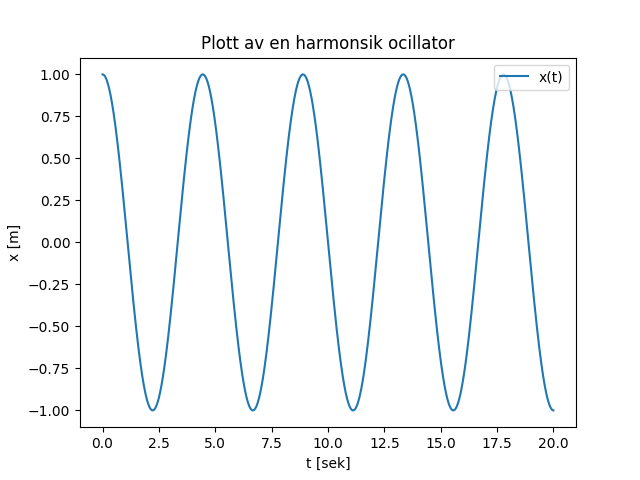
\includegraphics[width=12.6cm, height=7.7cm]{Prosjekt_1a.png}
\caption{Plott av løsningen til differensiallikningen. En harmonsik svigning som forventet.}
\label{1a}
			\end{figure}
			\begin{figure}[H]
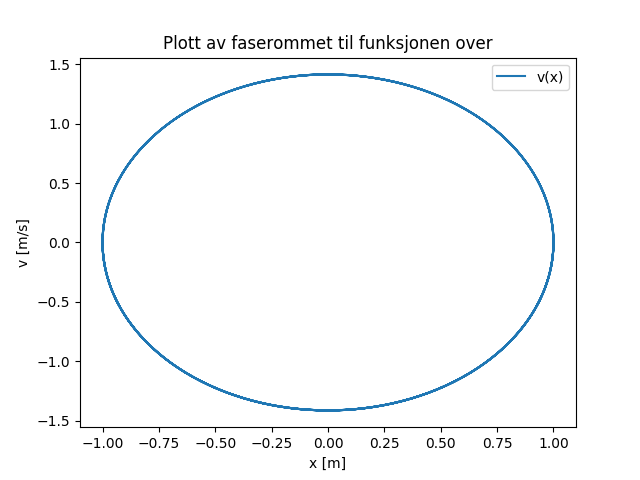
\includegraphics[width=12.6cm, height=7.7cm]{Prosjekt_1b.png}
\caption{Plott av faserommet til løsningen på differensiallikningen. Dette ble en ellipse.}
\label{1b}
			\end{figure}
			\begin{flushleft}
Det er ikke noe tap av energi i dette systemet, som vil si at det ikke er noen måter å få faseromet til ikke å se ut som en ellipse. Unntaket er hvis du setter startposisjon og starthastighet lik $0$. Da har ikke systemet noe energi i det hele tatt, og faserommet blir bare en strek. \\

Når det gjelder hvorfor banen i faserommet alltid står vinkelrett på $x$- og $y$-aksen kommer dette av at energien til systemet alltid er bevar. Et resultat av dette er at hastigheten og posisjonen til systemet alltid er maksimal når den andre er minimal. Dette kommer av sammenhengen
$$E_{\text{tot}} = E_{\text{kinetisk}} + E_{\text{potensiell}} = \frac{1}{2} m v^2 + \frac{1}{2} k x^2$$
Som tydelig gir at potensiell energi er størst når kinetisk energi er $0$ og omvendt. Dette gjør at hastigheten endrer stigningstall i det posisjonen er $0$, eller at posisjoen begynner å gå i motsatt retning når hastigheten er maksimal, dette kommer av at akselrasjonen til systemet alltid har motsatt fortegn av posisjonen. \\

Systemet i faserommet beveger seg med klokka, og så lenge differensiallikningen har det samme fortegnet vil det ikke spille noen rolle hva jeg gjør med initialbetingelsene for å prøve å endre retningen på faserommets bevegelse. Bevegelsen vil uansett være med klokka.
			\end{flushleft}








		\paragraph{2)}
			\begin{flushleft}
Inkluderer dempning i programmet ved å legge til leddet $- b / m * x$ i funksjoen som representerer differensiallikningen, med $b = 0.1 \text{kg/s}$. Importerer den Runge kutta $4$ funksjonen jeg lagde i forrige oppgave.
			\end{flushleft}
			\begin{figure}[H]
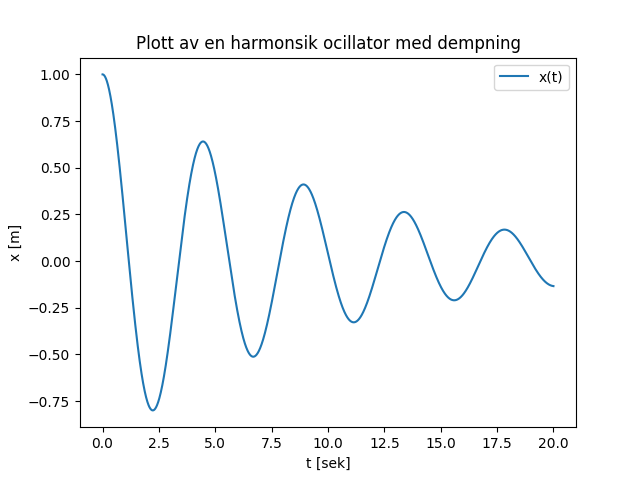
\includegraphics[width=12.6cm, height=7.7cm]{Prosjekt_2a.png}
\caption{Plott av løsningen til differensiallikningen med dempning.}
\label{2a}
			\end{figure}
			\begin{figure}[H]
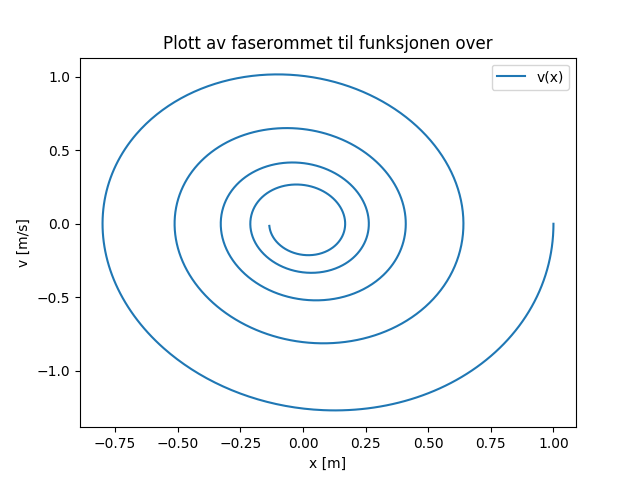
\includegraphics[width=12.6cm, height=7.7cm]{Prosjekt_2b.png}
\caption{Plott av faserommet til differensiallikningen med dempning.}
\label{2b}
			\end{figure}
			\begin{flushleft}
Plotter to plott akkurat som i forrige oppgave, det første av en svingebevegelse som blir stadig mindre \ref{2a}, og faserommet blir et sneilehus \ref{2b}. \\

Banen i faserommet står ikke lenger vinkelrett på begge aksene. I det nye plotte er det enkelt å se at det bare er $x$-aksen plottet står vinkelrett på. Dette kommer av at den kinetiske energien ikke lenger er maksimal når den potensielle energien er lik null. Dette kommer selvfølgelig av dempningen, som hele tiden senker den kinetiske energien. Derimot vil fortsatt den potensielle energien ha sine maksimale verdier hver gang hastigheten er null, siden dempingen da er null også. \\
Punktet $x(t) = 0$ og $x'(t) = 0$ kalles en attraktor fordi faserommet sin funksjon sakte men sikkert går mot dette punktet. \\

Dimensjonen til denne attraktoren er $0$ siden den er ett punkt. \\

Når det kommer til om kurva i oppgave $1$ er en attraktor så går denne kurva i en perfekt ellipse som alltid ender opp på samme sted. Det vil si at hvis en attraktor defineres som noe et system går mot, vil kurva ikke være det. Hvis en attraktor derimot er definert som noe et system ender opp som vil kurva være en attraktor.
			\end{flushleft}











		\paragraph{3)}
			\begin{gather*}
m \ddot{x}(t) + k x(t) = F_D \cos(\omega_D t) \\
\text{Løser denne differensiallikningen ved å legge sammen en homogen og en} \\
\text{partikulær løsning} \\
\ddot{x}(t) = - \frac{k}{m} x(t) \\
\text{Fra denne likningen er det lett å se at en løsning for dette blir} \\
x(t) = A \cos\left( \sqrt{\frac{k}{m}} t \right) + B \sin\left( \sqrt{\frac{k}{m}} t \right) \\
\text{Leter deretter etter en partikulær løsning på formen $C \cos(c t)$} \\
\text{Setter inn denne formen i likningen} \\
- m c^2 C \cos(c t) + k C \cos(c t) = F_D \cos( \omega_D t) \\
(k - m c^2)C \cos(c t) = F_D \cos(\omega_D t) \\
\text{Altså er} \\
c = \omega_D \\
C = \frac{F_D}{k - mc^2} = \frac{F_D}{k - m \omega_D^2} \\
x(t) = \frac{F_D}{k - m \omega_D^2} \cos\left( \omega_D t \right) \\
\text{Legger dette sammen og får} \\
x(t) = A \cos\left( \sqrt{\frac{k}{m}} t \right) + B \sin\left( \sqrt{\frac{k}{m}} t \right) + \frac{F_D}{k - m \omega_D^2} \cos\left( \omega_D t \right) \\
\text{Setter inn initialbetingelsene} \\
x(0) = A + \frac{F_D}{k - m \omega_D^2} = 2 \text{m} \Rightarrow A = 2 \text{m} - \frac{F_D}{k - m \omega_D^2} \\
\text{Skriver bare $2$ istedenfor $2 \text{m}$ etter dette} \\
\dot{x}(0) = \sqrt{\frac{k}{m}} B = 0 \Rightarrow B = 0 \\
x(t) = \left( 2 - \frac{F_D}{k - m \omega_D^2} \right) \cos\left( \sqrt{\frac{k}{m}} t \right) + \frac{F_D}{k - m \omega_D^2} \cos\left( \omega_D t \right) \\
x(t) = 2 \cos\left( \sqrt{\frac{k}{m}} t \right) + \frac{F_D}{k - m \omega_D^2} \left( \cos\left( \omega_D t \right) - \cos\left( \sqrt{\frac{k}{m}} t \right) \right) \\
			\end{gather*}
			\begin{gather*}
\text{Fra Rottmann \cite{Rot88} vet vi at dette kan skrives som} \\
x(t) = 2 \cos\left( \sqrt{\frac{k}{m}} t \right) + \frac{F_D}{k - m \omega_D^2} \left( - 2 \sin\left( \frac{\omega_D t + \sqrt{\frac{k}{m}} t}{2} \right) \sin\left( \frac{\omega_D t - \sqrt{\frac{k}{m}} t}{2} \right) \right) \\
x(t) = 2 \cos\left( \sqrt{\frac{k}{m}} t \right) - 2 \frac{F_D}{k - m \omega_D^2} \sin\left( \frac{\omega_D + \sqrt{\frac{k}{m}}}{2} t \right) \sin\left( \frac{\omega_D - \sqrt{\frac{k}{m}}}{2} t \right)
			\end{gather*}
			\begin{flushleft}
Jeg tolker dette som en del som den harmoniske svigningen, den første kosinusbølgen med amplitude $2 \text{m}$ og frekvens $\sqrt{\frac{k}{m}}$, og en påtrykt kraft som består av to sinusbølger multiplisert.
			\end{flushleft}			









		\paragraph{4)}
			\begin{flushleft}
Legger inn leddet $F_D \cos(\omega_D t)$ til differensiallikningsfunksjonen som ble brukt i oppgave $2$, og buker verdiene $F_D = 0.7 \text{N}$ og $\omega_D = \frac{13}{8} \omega_0 = \frac{13}{8} \sqrt{\frac{k}{m}}$. Endrer deretter på initialposisjoen til $x(0) = 2 \text{m}$ og sluttiden til $200 \text{s}$. Får som før to bilder.
			\end{flushleft}
			\begin{figure}[H]
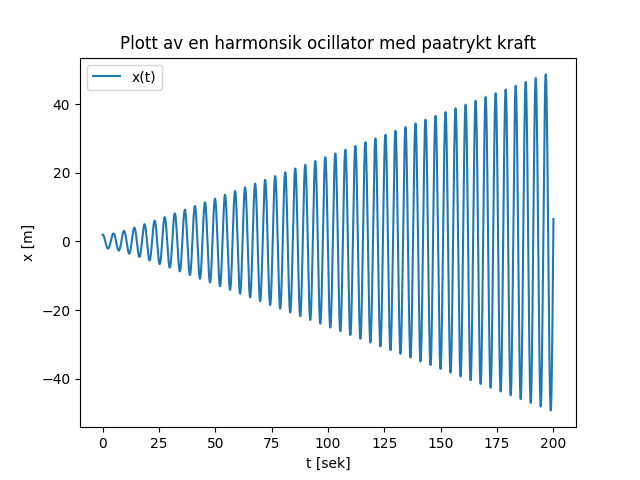
\includegraphics[width=12.6cm, height=7.7cm]{Prosjekt_4a.png}
\caption{Plott av en harmonisk ocillator med en påtrykt kraft.}
\label{4a}
			\end{figure}
			\begin{figure}[H]
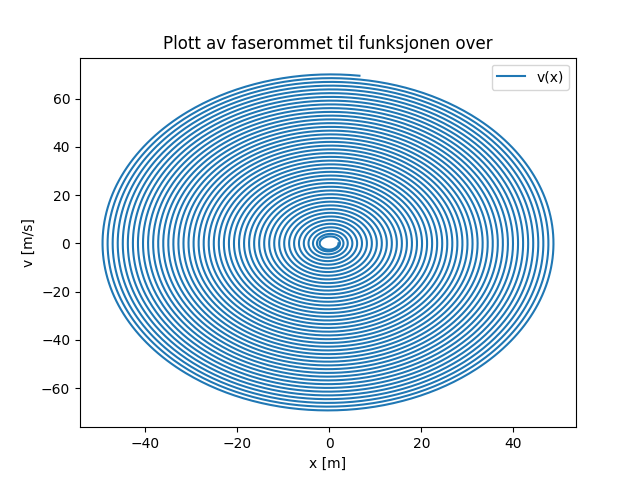
\includegraphics[width=12.6cm, height=7.7cm]{Prosjekt_4b.png}
\caption{Plott av faserommet til en harmonisk ocillator med en påtrykt kraft.}
\label{4b}
			\end{figure}
			\begin{flushleft}
Det første bildet viser en periodiske svigning som ser ut som en sinusbølge som med gradvis større amplitude \ref{4a}. Det andre bildet er av faserommet til den periodiske svigningen \ref{4b}. Her ser vi at i motsetning til i oppgave $2$ går ikke spiralen innover, men utover, bort fra origo.

Denne bevegelsen er periodisk, siden periodiske bevegelser er definert som bevegelse som gjentar seg med gjevne mellomrom i tid. Kurva paserer $x$-aksen men gjevne mellomrom i tid, og derfor er den periodisk \\

Lager en ny funksjon der jeg har byttet ut $\omega_D$ og gjennomfører Runge Kutta $4$ analysen igjen. Da får jeg to nye bilder som viser en bølge \ref{4c} og faserommet dens \ref{4d}.
			\end{flushleft}
			\begin{figure}[H]
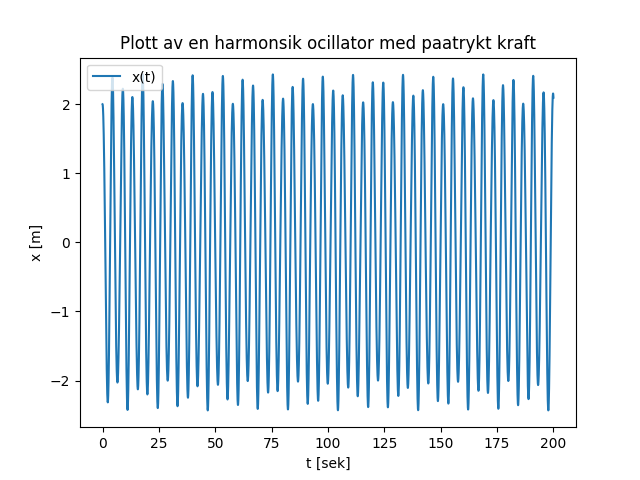
\includegraphics[width=12.6cm, height=7.7cm]{Prosjekt_4c.png}
\caption{Plott av en harmonisk ocillator med en påtrykt kraft.}
\label{4c}
			\end{figure}
			\begin{figure}[H]
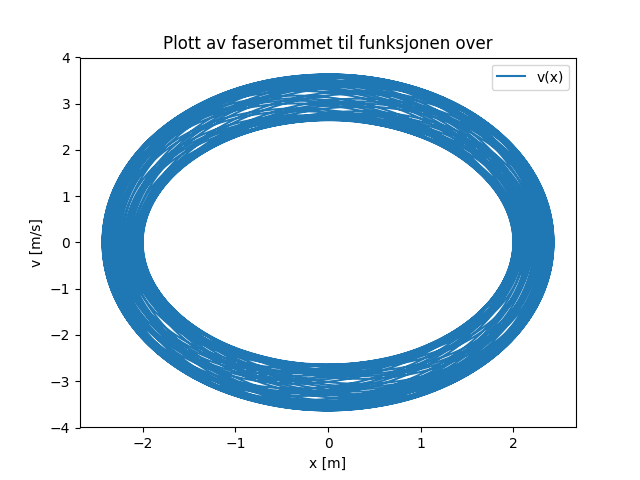
\includegraphics[width=12.6cm, height=7.7cm]{Prosjekt_4d.png}
\caption{Plott av faserommet til en harmonisk ocillator med en påtrykt kraft.}
\label{4d}
			\end{figure}
			\begin{flushleft}
Bølgen ser nå veldig mye mer kaotisk ut, men den er fortsatt periodisk fordi den passerer $x$-aksen med gjevne mellomrom fortsatt.
			\end{flushleft}











		\paragraph{5)}
			\begin{flushleft}
Legger så til demping på samme måte som tidligere. Fortsetter å bruke den første verdien for $\omega_D$.
			\end{flushleft}
			\begin{figure}[H]
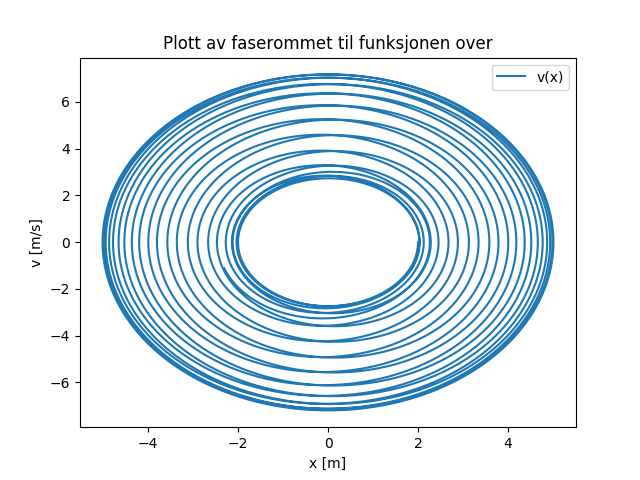
\includegraphics[width=12.6cm, height=7.7cm]{Prosjekt_5b.png}
\caption{Plott av faserommet til en harmonisk ocillator med en påtrykt kraft og dempning.}
\label{5b}
			\end{figure}
			\begin{flushleft}
Dette faserommet \ref{5b} er fortsatt veldig nærme å være sytematisk. Nå ser det ut til at faserommet roterer rundt origo mer eller mindre i gjevne sirkelbaner, selv om stedet der det er mest bevegelse er ute i en sirkel helt ytterst. Sånn som i oppgave $4$ ser det ut til at bevegelsen går mer og mer utover fra origo, men denne gangen er det ikke like systematisk. Formen er egentlig blitt mye nærmere det andre faserommet i oppgave $4$ \ref{4d}, altså en tykk ring. \\

Jo mer jeg øker verdien til dempningskonstanten, jo nærmere blir faserommet en sirkel, akkurat som hvis det ikke var noen dempning eller påtrykt kraft. Gjør jeg derimot konstanten mindre vil faserommet nærme seg slik det ser ut i oppgave $4$, akkurat som forventet siden det ikke vil være noen dempning hvis den var veldig liten.
			\end{flushleft}







		\paragraph{6)}
			\begin{flushleft}
Modifiserer differensiallikningsfuksjonen fra oppgave $1$ og bruker denne til å beregner likningssytemet som er oppgitt i oppgaven for å modelere vanndråpa, og plotter som tidligere både bevegelsen i tid- og faserommet.
			\end{flushleft}
			\begin{figure}[H]
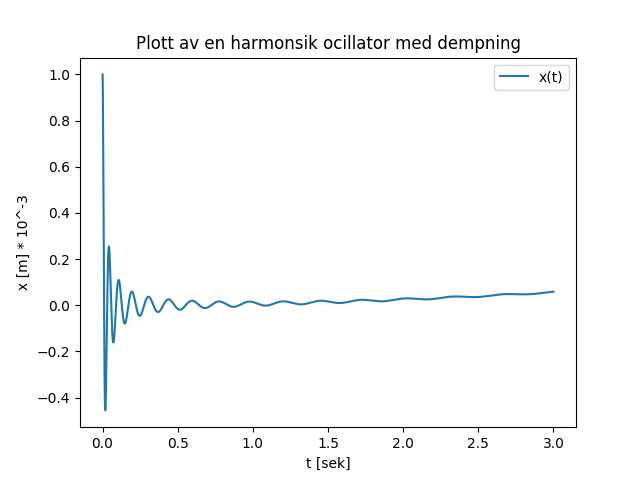
\includegraphics[width=12.6cm, height=7.7cm]{Prosjekt_6a.png}
\caption{Plott av modell for dråpe som henger i kran.}
\label{6a}
			\end{figure}
			\begin{figure}[H]
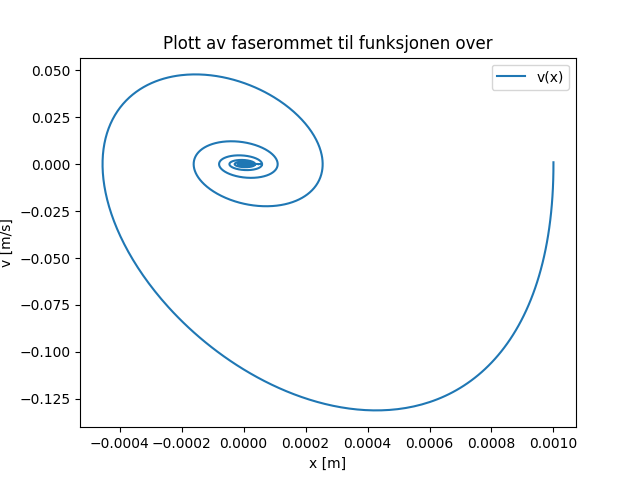
\includegraphics[width=12.6cm, height=7.7cm]{Prosjekt_6b.png}
\caption{Plott av faserommet til dråpemodellen.}
\label{6b}
			\end{figure}
			\begin{flushleft}
Hvis vi antar at modellen tar utgangspunkt i hinna på dråpa kan vi utifra plottet i tidrommet \ref{6a} se at dråpa sin hinne svinger ut fra krana og tilbake inn i den, og til slutt går mot å henge litt utafor krana, ikke stille men sakte men sikkert lenger og lenger unna krana. Dette er en ganske realistisk bevegelse av dråpa, selv om det kanskje ikke er så vanlig at dråpa beveger seg veldig mye tilbake opp i krana. \\

Fra faserommet ser vi at hastigheten også svinger mindre og mindre, mens hinna går mot kanten av krana.
			\end{flushleft}











		\paragraph{7)}
			\begin{flushleft}
Siden koden jeg brukte i oppgave $6$ importerer RK4 koden sin fra oppgave $1$ så er det denne koden jeg bruker. Forandrer denne slik at den endrer avstand og masse slik som beskrevet i oppgaven. Velger også å integrer over $21$ sekunder istedenfor over $20$. Etter at den første dråpen faller er det nesten helt konstant tid mellom hver dråpe som faller. Denne tiden er ca. ett og et halvt tidels sekund. Allikevel er det litt forskjell mellom dråpene noen ganger.
			\end{flushleft}
			\begin{figure}[H]
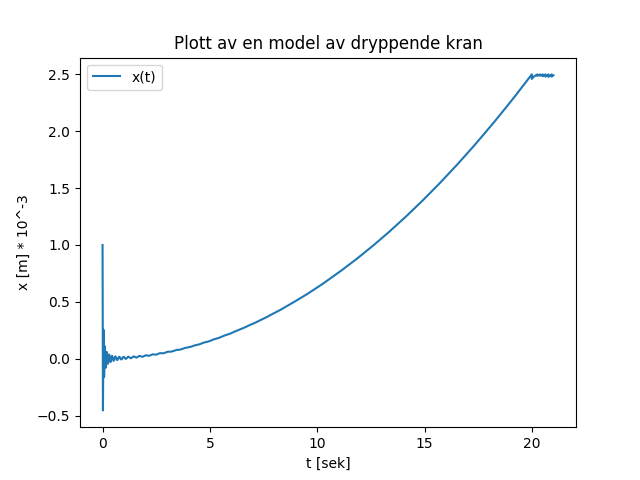
\includegraphics[width=12.6cm, height=7.7cm]{Prosjekt_7a.png}
\caption{Plott av faserommet til en modell for en dryppende kran.}
\label{7a}
			\end{figure}
			\begin{figure}[H]
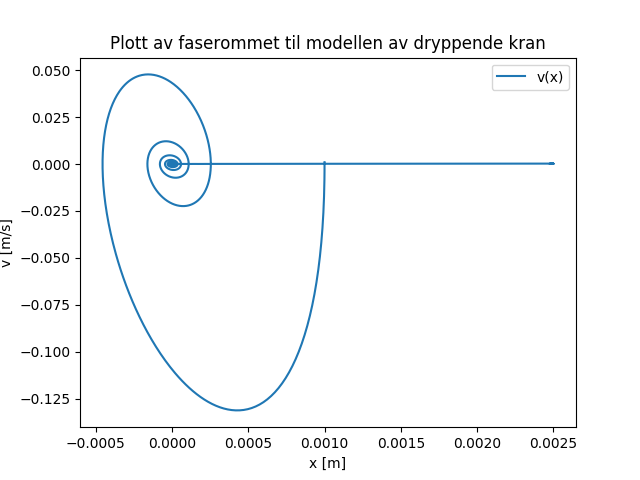
\includegraphics[width=12.6cm, height=7.7cm]{Prosjekt_7b.png}
\caption{Plott av faserommet til en modell for en dryppende kran.}
\label{7b}
			\end{figure}
			\begin{flushleft}
Prøvde å senke både starthastigheten og startposisjonen til $0$. Dette gjorde lite eller ingen forksjell, uten om å gjøre svigningen i starten mindre. Endret jeg massen til mindre blir svigningen i starten også mindre, og endrer jeg massen til større blir svigningen i starten lengre, men så lenger jeg ikke endrer noen parametere veldig mye ender alle resultatene opp med den samme dryppingen til slutt. \\

Ser vi på faserommet så er dette en spiral som veldig fort går inn mot $(0, 0)$ og deretter beveger seg mot høyre i en veldig lett sjelvende strek. Dette likner i starten på en veldig ekstrem versjon av faserommet i oppgave $2$, men streken har ikke noe med hverken faserom $4$ eller $2$. Denne streken gir uansett helt mening siden hastigheten til dråpehinna nå vil variere fra positiv til negativ hastighet veldig fort, slik at den ikke rekker å bli veldig stor. 
			\end{flushleft}










		\paragraph{8)}
			\begin{flushleft}
Legger inn nesten den samme RK4 fuksjonen som i forrige oppgaven, og legger inn nesten den samme funksjonen for differensiallikningen som jeg brukte i oppgave $6$. Eneste forskjellen er at jeg gjør det mulig å bestemme $\psi$-variabelen på forhånd av simulasjonen. Endrer så $\psi$ til hver av disse fire verdiene som er gitt i oppgaven. Det eneste dette gjør er at for hver endring blir det en lengre periode med drypping. Denne endringen blir mindre og mindre etterhvert som vi kommer nærmere $0.00075$ \ref{8a}.
			\end{flushleft}
			\begin{figure}[H]
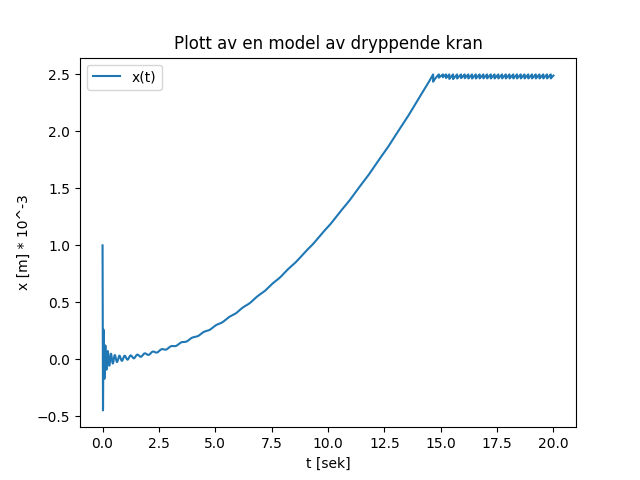
\includegraphics[width=12.6cm, height=9cm]{Prosjekt_8a.png}
\caption{Plott av samme modellen av dryppende kran som tidligere. $\psi$ er her lik $0.00075 \text{kg}/\text{s}$.}
\label{8a}
			\end{figure}
			\begin{flushleft}
Legger så til en test som regner ut og lagrer mellomrommene mellom de $50$ siste dråpene som faller. Dette fører til et veldig tregt program, men etter å ha gjort det, og plottet alle tidsverdiene mot en $\psi$, får jeg et bilde av en masse punkter som legger seg rundt akkurat de samme stedene  \ref{8c}. Disse punktene lager linjer som likner på sinus-/kosinusbølger. Variasjonen er mellom $0.26$ og $0.12$ sekunder. Noe som er en ganske lang forskjell egentlig, men det viser jo bare at det ikke nødvendigvis er et fullstendig konstant mellomrom mellom dråpene, men allikevel ganske likt mellomrom hele tiden. Kan ikke huske å ha spesifikt sett noe liknende noe annet sted, men det er jo bølger så har jo sett formene tidligere.
			\end{flushleft}
			\begin{figure}[H]
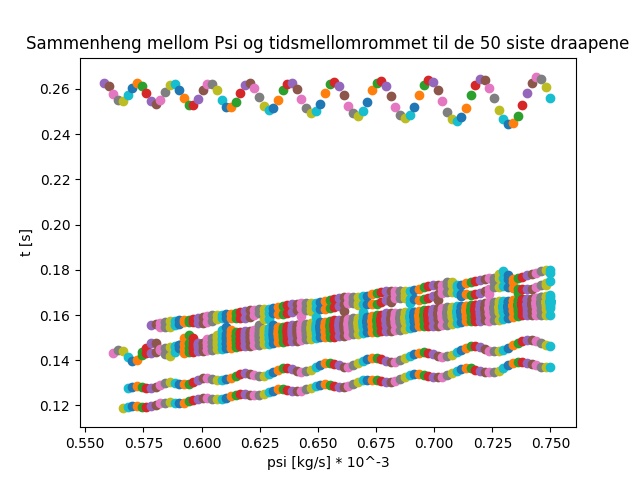
\includegraphics[width=12.6cm, height=9cm]{Prosjekt_8c.png}
\caption{Plott av sammenhengen til den siste dråpa som faller og masseøkningsraten, $\psi$.}
\label{8c}
			\end{figure}

			













		\paragraph{9)}
			\begin{flushleft}
Når det kommer til at jeg skal se på andre sitt arbeid med modeller for en dryppende kran så fant jeg en artikkel om å modellere systemet ved hjelp av en massefjær. Dette gir noen resultater som likner på mine. I denne artikkelen bruker de massesenteret til en dråpe som henger på krana og det er her i figur $4$ i artikkelen, \cite{Fig4_Tokyo} mulig å se at en dråpe slippes med gjevne mellomrom akkurat som vi finner og at dette skjer om og om igjen. Derimot viser deres figur en god del svigninger mellom hver gang det slippes en dråpe, noe som gir mening at skulle skje, men som ikke kommer frem i min model. \\

Ser jeg også på figur $3$ \cite{Fig3_Tokyo} ser jeg at tidsmellomrommene mellom hver av dråpene, plottet mot antall dråper, innretter seg i linjer akkurat som jeg får i plottet mitt i figur \ref{8c}. Jeg har ikke plottet tidsinterval mot antall dråper, men heller mot masseøkningsraten, men jo høyere masseøkningsraten er jo flere dråper faller, så tilfellen blir akkurat de samme.
			\end{flushleft}








		\begin{thebibliography}{9}
\bibitem{Rot88}
Karl Rottmann, side $88$. \\
\textit{Matematisk Formelsamling} \\
Bibliographisches Institut F. A Brockhaus, Estland, 2017.

\bibitem{Fig4_Tokyo}
Ken Kiyono og Nobuko Fuchikami, side $5$. \\
\textit{Dripping Faucet Dynamics Clarified by an Improved Mass-Spring Model} \\
Department of Physics, Tokyo Metropolitan University, Tokyo, 2017 \\
Lastet ned som PDF fra \url{https://arxiv.org/pdf/chao-dyn/9904012.pdf} den 07/05-2018

\bibitem{Fig3_Tokyo}
Ken Kiyono og Nobuko Fuchikami, side $4$. \\
\textit{Dripping Faucet Dynamics Clarified by an Improved Mass-Spring Model} \\
Department of Physics, Tokyo Metropolitan University, Tokyo, 2017 \\
Lastet ned som PDF fra \url{https://arxiv.org/pdf/chao-dyn/9904012.pdf} den 07/05-2018
		\end{thebibliography}
\end{document}